\chapter{Undecidability and Coping with Hardness}

NP-complete problems are believed to need exponential time, but they can at least be solved by brute force. Some problems cannot be solved
by \emph{any} algorithm at all.

\section{Decidability}
\begin{definition}
A decision problem is \textbf{decidable} if some algorithm (Turing machine, or program in any general-purpose language) halts on every input
and outputs the correct yes/no answer. Otherwise it is \textbf{undecidable}.
\end{definition}

A counting argument already shows undecidable problems exist: there are countably many programs (finite strings) but uncountably many
decision problems (subsets of $\{0,1\}^*$). The interesting fact is that natural problems are undecidable.

\section{The halting problem}
\textsc{Halt}: given (the source code of) a program $P$ and an input $x$, does $P$ halt on $x$?

\begin{theorem}[Turing 1936]
\textsc{Halt} is undecidable.
\end{theorem}
\begin{proof}
Suppose an algorithm $H(P,x)$ always halts and returns true iff $P$ halts on $x$. Write the program
\begin{lstlisting}[style=pseudo]
D(P):
    if H(P, P) then loop forever
    else return
\end{lstlisting}
Run $D$ on its own source. If $D(D)$ halts, then $H(D,D)$ is true, so $D(D)$ loops forever. If $D(D)$ loops forever, then $H(D,D)$ is false, so
$D(D)$ returns. Either way we have a contradiction, so $H$ cannot exist.
\end{proof}
This is a \emph{diagonalization} argument, like Cantor's proof that $\R$ is uncountable: $D$ differs from every program $P$ on input $P$.

\begin{figure}[H]
\centering
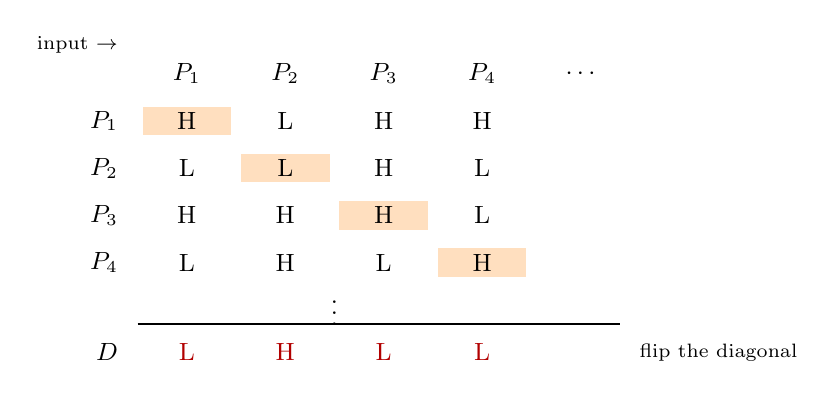
\begin{tikzpicture}[x=1.25cm, y=0.6cm, font=\small]
  \foreach \j in {1,...,4} \node at (\j,1) {$P_\j$};
  \node at (5,1) {$\cdots$};
  \node[font=\scriptsize, anchor=east] at (0.4,1.6) {input $\to$};
  \foreach \i/\row in {1/{H,L,H,H}, 2/{L,L,H,L}, 3/{H,H,H,L}, 4/{L,H,L,H}} {
    \node[anchor=east] at (0.4,-\i+1) {$P_\i$};
    \foreach \v [count=\j] in \row {
      \ifnum\i=\j \fill[orange!25] (\j-0.45,-\i+0.7) rectangle (\j+0.45,-\i+1.3); \fi
      \node at (\j,-\i+1) {\v};
    }
  }
  \node at (2.5,-3.9) {$\vdots$};
  \draw[thick] (0.5,-4.3) -- (5.4,-4.3);
  \node[anchor=east] at (0.4,-4.9) {$D$};
  \foreach \v [count=\j] in {L,H,L,L} \node[red!70!black] at (\j,-4.9) {\v};
  \node[font=\scriptsize, anchor=west] at (5.5,-4.9) {flip the diagonal};
\end{tikzpicture}
\caption{Entry $(i,j)$ records whether $P_i$ halts (H) or loops (L) on input
$P_j$. $D$ does the opposite of the diagonal, so it differs from every
$P_i$ on input $P_i$ and cannot appear as any row.}
\end{figure}

\section{Reductions for undecidability}
If $A$ is undecidable and $A\le B$ via a \emph{computable} (not necessarily polynomial) map $f$ with $x\in A\iff f(x)\in B$, then $B$ is undecidable;
otherwise a decider for $B$ composed with $f$ would decide $A$. Turing reductions (deciding $A$ using a hypothetical decider for $B$ as a subroutine) work too.

\begin{example}[Halting on empty input]
\textsc{Halt-}$\varepsilon$: does $P$ halt on the empty input? Reduce from \textsc{Halt}: given $(P,x)$, build $P_x$ that ignores its input and runs $P$ on $x$
(hard-code $x$). Then $P_x$ halts on $\varepsilon$ iff $P$ halts on $x$.
\end{example}

\begin{example}[Program equivalence]
\textsc{Equiv}: do programs $P_1,P_2$ produce the same output on every input? Reduce from \textsc{Halt-}$\varepsilon$: given $P$, let
$P_1(y)$ = ``run $P$ on $\varepsilon$, then output 1'' and $P_2(y)$ = ``output 1''. They are equivalent iff $P$ halts on $\varepsilon$.
\end{example}

\begin{example}[Does $P$ ever output 0?]
Given $P$, build $Q(y)$ = ``run $P$ on $\varepsilon$; output 0''. $Q$ ever outputs 0 iff $P$ halts on $\varepsilon$.
\end{example}

\begin{theorem}[Rice's theorem, statement]
Every nontrivial property of the \emph{function computed} by a program (true for some programs and false for others, depending only on the input/output behaviour)
is undecidable.
\end{theorem}
Other undecidable problems: Hilbert's tenth problem (does a polynomial equation with integer coefficients have an integer solution?), Post's correspondence problem,
whether a context-free grammar is ambiguous, and tiling the plane with a given set of Wang tiles.

\begin{important}[Hierarchy]
\[
\mathbf P\subseteq\mathbf{NP}\subseteq\mathbf{PSPACE}\subseteq\mathbf{EXP}\subsetneq\text{decidable}\subsetneq\text{all problems}.
\]
NP-complete problems are decidable (in exponential time); \textsc{Halt} is not decidable at all. Note that \textsc{Halt} is NP-hard
(any decidable problem reduces to it), but it is not in NP.
\end{important}

\begin{figure}[H]
\centering
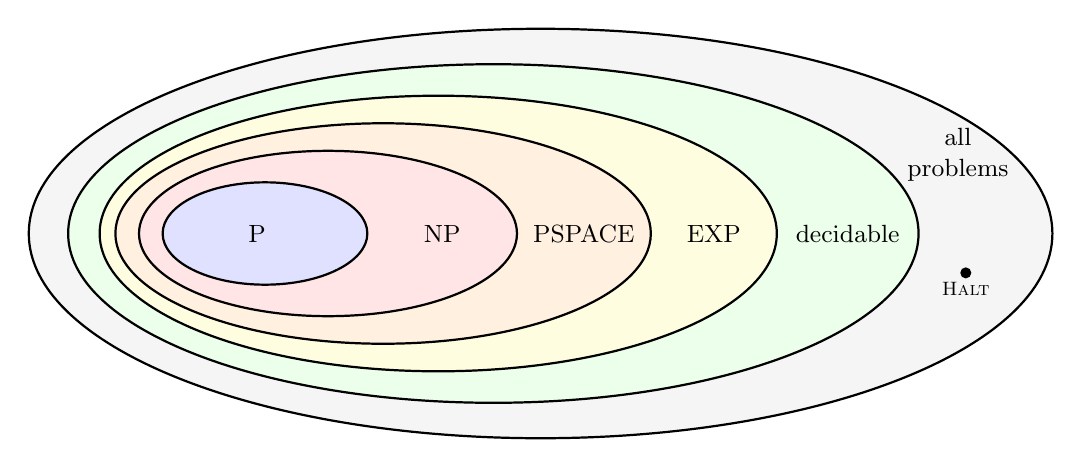
\begin{tikzpicture}[font=\small]
  \draw[thick, fill=gray!8] (0,0) ellipse (6.5 and 2.6);
  \draw[thick, fill=green!8] (-0.6,0) ellipse (5.4 and 2.15);
  \draw[thick, fill=yellow!12] (-1.3,0) ellipse (4.3 and 1.75);
  \draw[thick, fill=orange!12] (-2.0,0) ellipse (3.4 and 1.4);
  \draw[thick, fill=red!10] (-2.7,0) ellipse (2.4 and 1.05);
  \draw[thick, fill=blue!12] (-3.5,0) ellipse (1.3 and 0.65);
  \node at (-3.6,0) {P};
  \node at (-1.25,0) {NP};
  \node at (0.55,0) {PSPACE};
  \node at (2.2,0) {EXP};
  \node at (3.9,0) {decidable};
  \node[align=center] at (5.3,1.0) {all\\problems};
  \fill (5.4,-0.5) circle (2pt) node[below, font=\scriptsize]{\textsc{Halt}};
\end{tikzpicture}
\caption{The hierarchy of problem classes (only $\mathbf{EXP}\subsetneq$
decidable and the outer inclusion are known to be strict).}
\end{figure}

\section{Coping with NP-hardness}
Showing a problem is NP-complete does not mean we give up. Options:

\subsection{Special cases}
Restricted inputs may be easy: Independent Set on trees or interval graphs (greedy/DP), 2-SAT (via SCCs of the implication graph, linear time),
2-colouring (BFS), Vertex Cover on bipartite graphs (matching), knapsack with small $W$ (pseudo-polynomial DP).

\subsection{Exact exponential algorithms}
Do better than brute force:
\begin{itemize}
  \item \textbf{Backtracking / branch and bound}: explore partial solutions, prune those that cannot lead to a solution or beat the best found so far.
  \item \textbf{DP over subsets}: Held--Karp solves TSP in $\bigO(n^22^n)$ instead of $\bigO(n!)$, with $D[S][v]$ = shortest path from $1$ visiting exactly $S$ and ending at $v$:
        $D[S][v]=\min_{u\in S\setminus\{v\}}D[S\setminus\{v\}][u]+w(u,v)$.
  \item \textbf{Fixed-parameter tractability}: Vertex Cover of size $k$ in $\bigO(2^k m)$: pick any edge $uv$; one of $u,v$ is in the cover, so branch on both, recursing with $k-1$.
        Depth $k$, branching factor 2.
\end{itemize}

\subsection{Approximation algorithms}
An $\alpha$-approximation (for minimization) runs in polynomial time and always returns a solution of cost $\le\alpha\cdot\mathrm{OPT}$.
\begin{itemize}
  \item \textbf{Vertex Cover, factor 2}: repeatedly pick an uncovered edge $uv$ and add both $u$ and $v$. The picked edges form a matching $M$; any cover contains an
        endpoint of each matching edge, so $\mathrm{OPT}\ge|M|$, while we output $2|M|$.
  \item \textbf{Metric TSP, factor 2}: compute an MST $T$ (Chapter 7), walk around it (each edge twice), and shortcut repeated vertices. Removing one edge of an optimal tour
        gives a spanning tree, so $w(T)\le\mathrm{OPT}$; the walk costs $2w(T)$ and shortcuts don't increase cost by the triangle inequality. (Christofides improves this to $3/2$.)

\begin{figure}[H]
\centering
\begin{tikzpicture}[x=0.85cm, y=0.85cm, >=Stealth,
  pt/.style={circle, fill=black, inner sep=1.6pt}]
  \foreach \c/\title in {0/{MST $T$}, 5.5/{walk around $T$}, 11/{shortcut tour}} {
    \begin{scope}[xshift=\c cm]
      \node[font=\small] at (2,3.4) {\title};
      \foreach \n/\x/\y in {a/2/2.8, b/0.6/1.6, c/3.4/1.8, d/0/0, e/1.4/0.2, f/3.8/0.2}
        \node[pt] (\n\c) at (\x,\y) {};
    \end{scope}
  }
  \foreach \u/\v in {a/b, a/c, b/d, b/e, c/f} \draw[very thick, blue!60!black] (\u0) -- (\v0);
  \node[font=\scriptsize, above] at (a0.north) {$r$};
  \begin{scope}[xshift=5.5cm]
    \draw[->, thick, gray!70!black, rounded corners=4pt]
      (2,2.95) -- (0.45,1.75) -- (-0.15,0.05) -- (0.55,1.45) -- (1.5,0.05) -- (0.75,1.55)
      -- (2.05,2.6) -- (3.45,1.65) -- (3.75,0.05) -- (3.55,1.95) -- (2.1,2.95);
  \end{scope}
  \foreach \u/\v in {a/b, b/d, d/e, e/c, c/f, f/a} \draw[very thick, red!70!black] (\u11) -- (\v11);
\end{tikzpicture}
\caption{The 2-approximation for metric TSP: a walk around the MST from
$r$ traverses each tree edge twice; skipping already-visited vertices
(shortcutting) gives the tour $r, \ldots$ visiting the vertices in DFS
order, which is no longer than the walk.}
\end{figure}
  \item \textbf{General TSP} has no constant-factor approximation unless $\mathbf P=\mathbf{NP}$: with weights 1 for edges and $\alpha n+1$ for non-edges, an $\alpha$-approximation would decide Ham-Cycle.
  \item \textbf{Knapsack} has an FPTAS: scale and round values, then run the value-indexed DP, giving $(1-\varepsilon)$-optimal solutions in time polynomial in $n$ and $1/\varepsilon$.
\end{itemize}

\subsection{Heuristics}
Local search, simulated annealing, SAT solvers, integer programming solvers: no worst-case guarantees but often excellent in practice.

\section*{Summary}
\begin{itemize}
  \item \textsc{Halt} is undecidable by diagonalization; reductions (computable maps) spread undecidability.
  \item Undecidable is strictly worse than NP-complete: NP-complete problems are solvable in exponential time.
  \item Coping with NP-hardness: special cases, smarter exponential algorithms (Held--Karp, FPT), approximation (2-approx VC and metric TSP), heuristics.
\end{itemize}
